\chapter{\MakeUppercase{Tinjauan Pustaka}}

Bab ini memuat kajian teoritis yang menjadi landasan dalam pelaksanaan penelitian. Uraian yang disajikan harus merupakan hasil pemahaman, analisis, dan sintesis penulis terhadap berbagai sumber pustaka yang relevan, bukan sekadar penyalinan ulang isi referensi.

Tinjauan pustaka berisi pembahasan mengenai teori, konsep, metode, algoritma, pendekatan, model, maupun sistem yang berkaitan dengan topik penelitian. Pembahasan difokuskan pada prinsip-prinsip ilmiah yang mendasari penelitian, bukan pada uraian spesifikasi teknis perangkat tertentu, seperti papan pengembangan (*development board*), komponen elektronik, sensor, aktuator, maupun perangkat keras lainnya.

Bab ini disusun berdasarkan beberapa bidang ilmu atau topik utama yang relevan dengan penelitian. Setiap bidang ilmu dipilih berdasarkan keterkaitannya dengan sistem yang diusulkan dan dibedakan berdasarkan ruang lingkup serta batasan pembahasannya. Jumlah topik yang dibahas umumnya berkisar antara tiga hingga lima bidang ilmu utama, sesuai kebutuhan penelitian.

Untuk setiap topik yang dibahas, uraian sebaiknya mencakup hal-hal berikut:

\begin{enumerate}[topsep=0pt,itemsep=0pt,parsep=0pt,leftmargin=*]
\item Penjelasan mengenai konsep, teori, metode, atau pendekatan yang digunakan.
\item Hubungan teori tersebut dengan teori lain, termasuk asal-usul pengembangannya maupun arah pengembangannya lebih lanjut.
\item Deskripsi mengenai metode, algoritma, atau sistem yang dibahas, meliputi:
\begin{itemize}[topsep=0pt,itemsep=0pt,parsep=0pt,leftmargin=*]
\item struktur atau tahapan algoritma/sistem;
\item komponen-komponen penyusun;
\item diagram atau model sistem;
\item prinsip dan mekanisme kerja.
\end{itemize}
\item Bidang atau kasus penerapan yang umum menggunakan teori, metode, atau sistem tersebut.
\item Kesesuaian teori, metode, konfigurasi, atau komponen yang dipilih dengan kebutuhan penelitian yang dilakukan.
\end{enumerate}

Pembahasan dalam bab ini sebaiknya disusun secara sistematis, dimulai dari konsep yang bersifat umum menuju konsep yang lebih spesifik, sehingga membentuk landasan yang kuat bagi pengembangan solusi dan metodologi penelitian pada bab-bab berikutnya.

\section{Pedoman Bahasa dan Penulisan Ilmiah}
\subsection{Kesalahan Umum dalam Penggunaan Bahasa Indonesia pada Penulisan Tugas Akhir}

Dalam penyusunan tugas akhir, terdapat beberapa kesalahan yang sering dijumpai dan perlu dihindari. Kesalahan-kesalahan tersebut dapat mengurangi kejelasan, keterbacaan, serta kualitas ilmiah naskah yang disusun \cite{PUEBI2022, ArifinTasai2014}.

\begin{itemize}[topsep=0pt,itemsep=0pt,parsep=0pt,leftmargin=*]
\item Menulis kalimat yang terlalu panjang dan kompleks sehingga hubungan antara subjek, predikat, objek, dan keterangan menjadi tidak jelas. Kondisi ini sering terjadi akibat penggunaan kata penghubung, seperti “yang”, secara berlebihan. Sebaiknya, gunakan kalimat yang sederhana, lengkap, dan mudah dipahami. Setiap kalimat idealnya memiliki struktur SPOK (Subjek, Predikat, Objek, dan Keterangan) yang jelas.

\item Menggunakan kalimat yang bertele-tele atau tidak langsung pada inti pembahasan. Penulisan ilmiah sebaiknya menggunakan kalimat efektif, yaitu kalimat yang menyampaikan informasi secara jelas, ringkas, dan tepat tanpa penggunaan kata-kata yang tidak diperlukan.

\item Menulis kalimat yang tidak memiliki subjek atau predikat yang jelas. Kalimat semacam ini umumnya hanya berupa frasa sehingga tidak dapat menyampaikan gagasan secara utuh.

\item Menggunakan tanda baca secara kurang tepat. Kesalahan penempatan tanda baca dapat mengubah makna kalimat atau mengganggu keterbacaan naskah. Oleh karena itu, penggunaan tanda baca harus mengikuti kaidah Bahasa Indonesia yang berlaku.

\item Menggunakan istilah asing secara tidak konsisten atau menggabungkan istilah asing dan istilah Bahasa Indonesia dalam konteks yang sama sehingga menimbulkan ambiguitas dan kebingungan bagi pembaca.

\item Menyusun kalimat yang sulit dipahami akibat struktur kalimat yang terlalu rumit, penggunaan istilah yang berlebihan, atau kurangnya kejelasan dalam penyampaian ide.
\end{itemize}

\subsection{Penggunaan Istilah Asing}
Dokumen teknis dan karya ilmiah pada umumnya memuat banyak istilah khusus yang berasal dari berbagai bidang ilmu. Dalam bidang teknik, khususnya teknik elektro, komputer, telekomunikasi, dan fisika, penggunaan istilah asing sering kali tidak dapat dihindari.

Apabila suatu istilah telah memiliki padanan yang baku dalam Bahasa Indonesia, maka penggunaan padanan tersebut lebih diutamakan. Namun demikian, apabila padanan yang tersedia kurang umum digunakan atau berpotensi menimbulkan kesalahpahaman, istilah asing dapat tetap digunakan.

Penulis perlu berhati-hati dalam mengadopsi istilah asing ke dalam Bahasa Indonesia. Sebagai contoh, penggunaan kata “eksisting” sebagai terjemahan langsung dari kata *existing* sering dijumpai dalam karya ilmiah, padahal dalam banyak konteks kata tersebut dapat digantikan dengan istilah yang lebih tepat, seperti “saat ini”, “yang sudah ada”, atau “yang telah tersedia”.

Untuk memastikan ketepatan penggunaan istilah Bahasa Indonesia, penulis disarankan merujuk pada \gls{kbbi} \cite{KBBI2026} atau sumber rujukan bahasa yang kredibel.

Istilah asing atau istilah teknis yang belum memiliki padanan yang umum digunakan dalam Bahasa Indonesia dapat dituliskan dalam bahasa aslinya dengan format \textit{italic}. Penggunaan istilah tersebut harus dilakukan secara konsisten di seluruh dokumen agar tidak menimbulkan kebingungan bagi pembaca.

\section{Format Penulisan Tugas Akhir}

Tampilan dokumen merupakan salah satu aspek penting dalam penyusunan tugas akhir karena berpengaruh terhadap keterbacaan, kerapian, dan keseragaman naskah. Oleh karena itu, penulisan tugas akhir harus mengikuti format yang telah ditetapkan~\cite{panduanTA2017}. Beberapa ketentuan yang perlu diperhatikan dijelaskan sebagai berikut.

\subsection{Kertas}

Naskah tugas akhir dicetak menggunakan kertas HVS berwarna putih dengan berat 80 gram/m$^2$ dan ukuran A4 (21,0 cm $\times$ 29,7 cm).

\subsection{Pengetikan}

Pengetikan dan pencetakan naskah dilakukan pada satu sisi kertas (\textit{single-sided printing}). Batas tepi halaman yang digunakan mengacu pada Tabel~\ref{tab:pengetikan}.

\begin{table}[!ht]
\centering
\caption{Batas tepi halaman untuk penulisan tugas akhir}
\label{tab:pengetikan}
\begin{tabular}{|c|c|p{0.5\textwidth}|}
\hline
\textbf{Tepi Halaman} & \textbf{Jarak (cm)} & \textbf{Keterangan} \\
\hline
Kiri & 4 & Termasuk ruang untuk proses penjilidan \\
\hdashline
Kanan & 3 & -- \\
\hdashline
Atas & 3 & -- \\
\hdashline
Bawah & 3 & -- \\
\hline
\end{tabular}
\end{table}

Naskah diketik menggunakan huruf Times New Roman ukuran 12 pt. Bagi pengguna \LaTeX, jenis huruf tersebut dapat diperoleh menggunakan paket \texttt{mathptmx}. Seluruh isi naskah ditulis dengan perataan kiri-kanan (\textit{justify}) dan menggunakan spasi 1,5. Warna huruf yang digunakan harus hitam dan tercetak secara jelas serta seragam.

\subsection{Penomoran Halaman}

Penomoran halaman menggunakan dua jenis angka, yaitu angka Romawi kecil dan angka Arab.

Angka Romawi kecil (i, ii, iii, dan seterusnya) digunakan untuk bagian awal tugas akhir, kecuali halaman sampul. Nomor halaman ditempatkan di tengah bagian bawah halaman dengan jarak 2,5 cm dari tepi bawah kertas. Halaman judul tidak menampilkan nomor halaman, tetapi tetap diperhitungkan dalam penomoran.

Angka Arab (1, 2, 3, dan seterusnya) digunakan untuk bagian isi dan bagian akhir tugas akhir, termasuk daftar pustaka. Nomor halaman ditempatkan di sudut kanan atas dengan jarak 1,5 cm dari tepi atas dan 3 cm dari tepi kanan halaman.

Khusus pada halaman pertama setiap bab, nomor halaman ditempatkan di tengah bagian bawah halaman dengan jarak 2,5 cm dari tepi bawah kertas.

\subsection{Ketentuan Halaman Sampul}

Seluruh informasi pada halaman sampul ditulis secara simetris dan ditempatkan di tengah halaman (\textit{centered}).

Judul tugas akhir harus ditulis secara jelas dan ringkas serta tidak menggunakan singkatan, kecuali singkatan atau istilah yang telah umum digunakan pada bidang keilmuan terkait, seperti MIMO, WLAN, atau IoT. Judul tidak ditulis dalam bentuk kalimat tanya dan tidak diakhiri dengan tanda baca.

\section{Penyisipan Gambar, Tabel, dan Persamaan}

\subsection{Gambar}

Setiap gambar harus diberi nomor urut dan judul yang ditempatkan di bawah gambar. Penomoran gambar mengikuti format nomor bab dan nomor urut gambar pada bab tersebut.

Sebagai contoh, Gambar~\ref{fig:audioanomaly} menunjukkan konsep pendeteksian anomali berbasis audio.

\begin{figure}[!ht]
\centering
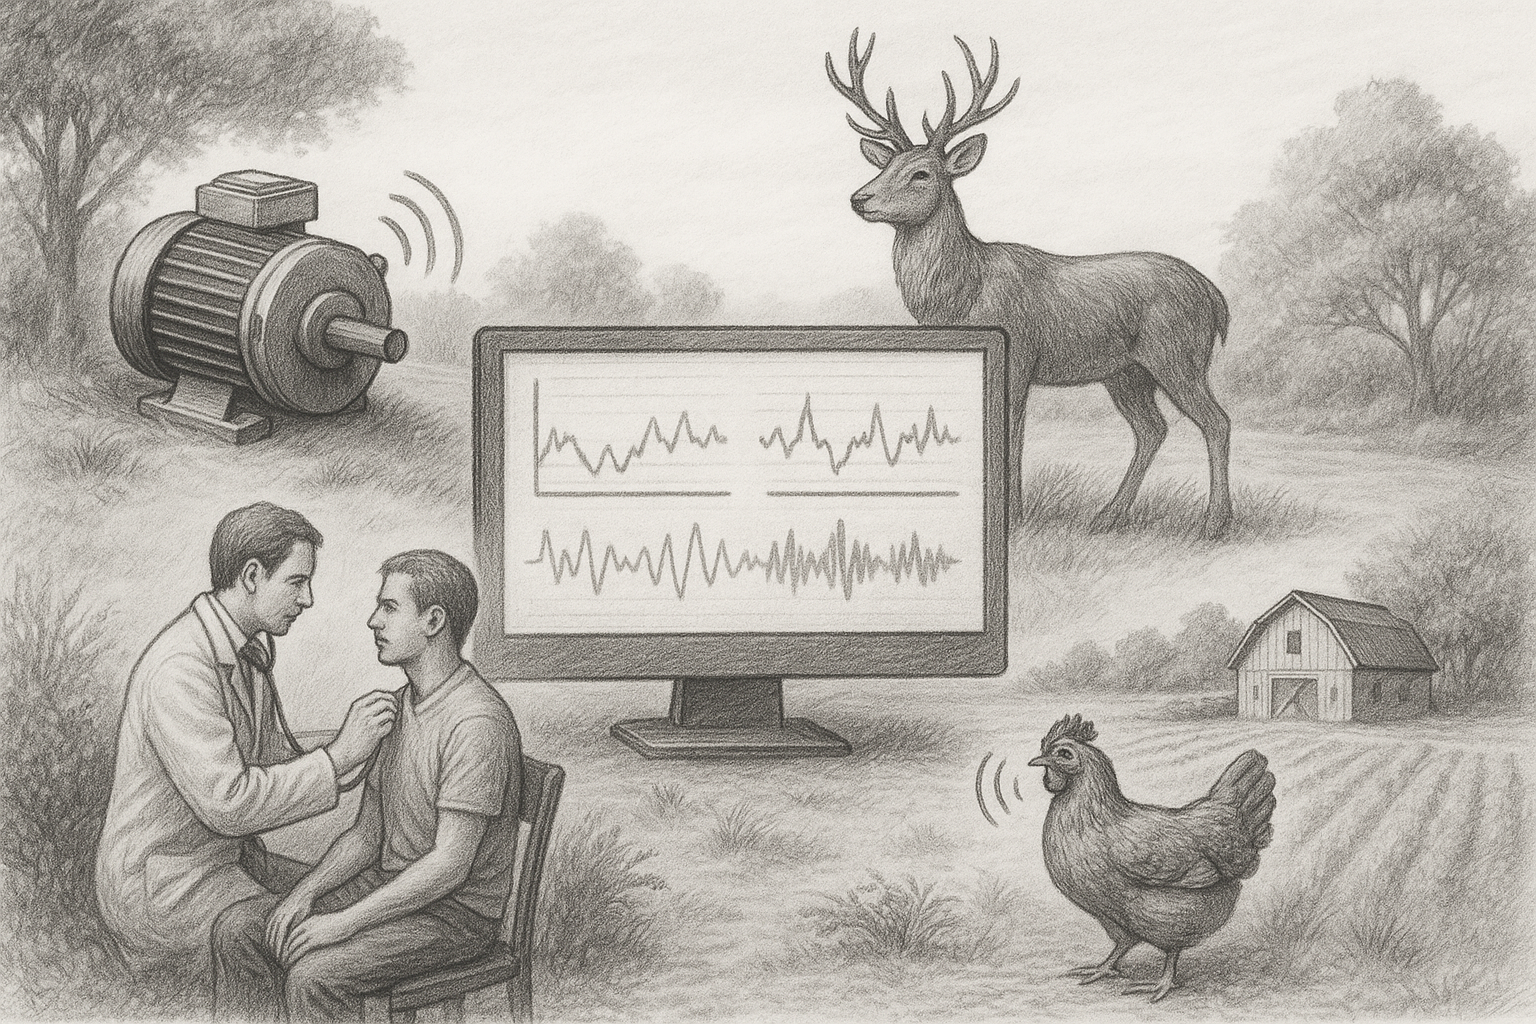
\includegraphics[width=0.75\linewidth]{Gambar/AudioBasedAnomalyDetection.png}
\caption{Konsep pendeteksian anomali berbasis audio}
\label{fig:audioanomaly}
\end{figure}

Setiap gambar yang disisipkan harus dirujuk dalam uraian naskah, baik sebelum maupun sesudah gambar ditampilkan. Selain itu, harus terdapat penjelasan yang memadai mengenai isi gambar, tujuan penyisipannya, serta keterkaitannya dengan pembahasan.

\subsection{Tabel}

Setiap tabel harus diberi nomor urut dan judul yang ditempatkan di atas tabel. Penomoran tabel mengikuti format nomor bab dan nomor urut tabel pada bab tersebut.

Sebagai contoh, karakteristik hubungan antara masukan dan keluaran suatu sistem dapat disajikan seperti pada Tabel~\ref{tab:hubungan}.

\begin{table}[!ht]
\centering
\caption{Hubungan antara masukan dan keluaran}
\label{tab:hubungan}
\begin{tabular}{|c|c|c|c|}
\hline
No. & Masukan 1 & Masukan 2 & Keluaran \\
\hline
1 & A & A & C \\
2 & A & B & D \\
3 & B & A & E \\
4 & B & B & F \\
\hline
\end{tabular}
\end{table}

Setiap tabel harus dirujuk dalam teks dan disertai penjelasan mengenai isi tabel, makna data yang disajikan, serta relevansinya terhadap pembahasan.

\subsection{Persamaan}

Persamaan matematis digunakan untuk menjelaskan hubungan antarvariabel, parameter, atau besaran yang digunakan dalam penelitian. Persamaan harus ditulis menggunakan lingkungan \texttt{equation} atau lingkungan lain yang sesuai dari paket \texttt{amsmath}.

Setiap persamaan yang akan dirujuk pada bagian lain naskah harus diberi label menggunakan perintah \verb|\label{}| sehingga nomor persamaan dapat dikelola secara otomatis dan konsisten.

Sebagai contoh, kode berikut:

\begin{tcolorbox}
\verb|\begin{equation}|
\verb|E = mc^2|
\verb|\label{eq:einstein}|
\verb|\end{equation}|
\end{tcolorbox}

akan menghasilkan Persamaan~(\ref{eq:einstein}).

\begin{equation}
E = mc^2
\label{eq:einstein}
\end{equation}

Setiap persamaan yang disajikan harus dirujuk dan dijelaskan dalam uraian naskah. Penjelasan tidak hanya mencakup tujuan penggunaan persamaan, tetapi juga arti setiap variabel, parameter, konstanta, dan satuan yang digunakan.

Sebagai contoh, apabila digunakan persamaan energi relativistik pada Persamaan~(\ref{eq:einstein}), maka penjelasan simbol-simbol yang digunakan dapat dituliskan sebagai berikut:

\begin{itemize}[topsep=0pt,itemsep=0pt,parsep=0pt,leftmargin=*]
\item $E$ adalah energi (Joule);
\item $m$ adalah massa benda (kg);
\item $c$ adalah kecepatan cahaya di ruang hampa ($\approx 3 \times 10^8$ m/s).
\end{itemize}

Penjelasan variabel dapat dituliskan dalam bentuk daftar, paragraf, maupun tabel sesuai dengan jumlah simbol yang digunakan. Untuk persamaan yang kompleks dan melibatkan banyak parameter, penggunaan tabel simbol lebih disarankan agar lebih mudah dibaca.

Beberapa ketentuan yang perlu diperhatikan dalam penulisan persamaan adalah sebagai berikut:

\begin{itemize}[topsep=0pt,itemsep=0pt,parsep=0pt,leftmargin=*]
\item Setiap persamaan harus dirujuk dalam teks sebelum atau sesudah persamaan ditampilkan.
\item Simbol, variabel, parameter, dan konstanta yang muncul pada persamaan harus dijelaskan ketika pertama kali digunakan.
\item Satuan setiap variabel atau parameter perlu dicantumkan apabila relevan.
\item Notasi yang digunakan harus konsisten di seluruh dokumen.
\item Simbol matematika ditulis menggunakan mode matematika (\textit{math mode}).
\item Persamaan yang diambil dari referensi lain harus mencantumkan sumber rujukan yang sesuai.
\end{itemize}

\section{Penulisan Kutipan Format IEEE}

Penggunaan kutipan dalam penulisan karya ilmiah bertujuan untuk mendukung argumentasi, memperkuat landasan teori, serta menunjukkan keterkaitan penelitian dengan karya ilmiah yang telah dipublikasikan sebelumnya. Meskipun demikian, isi naskah sebaiknya tetap didominasi oleh hasil analisis, pemikiran, dan kontribusi penulis, sehingga tidak menjadi kumpulan kutipan dari berbagai sumber.

Dalam penulisan tugas akhir, penggunaan kutipan perlu dilakukan secara proporsional dan relevan dengan konteks pembahasan. Penulis disarankan untuk lebih banyak menggunakan kutipan tidak langsung dibandingkan kutipan langsung agar alur penulisan tetap mengedepankan hasil sintesis dan pemahaman penulis terhadap sumber yang dirujuk. Setiap kutipan harus memberikan nilai tambah terhadap pembahasan dan mendukung pengembangan gagasan penelitian.

Berdasarkan cara penyajiannya, kutipan dapat dibedakan menjadi dua jenis sebagai berikut.

\begin{description}
    \item[Kutipan langsung] yaitu kutipan yang ditulis persis sama dengan sumber aslinya tanpa mengubah susunan kata, ejaan, maupun tanda baca. Kutipan langsung digunakan apabila redaksi asli sumber dianggap penting untuk dipertahankan.
    
    \item[Kutipan tidak langsung] yaitu kutipan yang memuat ide, konsep, atau hasil pemikiran dari sumber lain yang disampaikan kembali menggunakan kalimat dan gaya bahasa penulis sendiri tanpa mengubah makna aslinya.
\end{description}

Pada format sitasi \gls{ieee}, sumber rujukan dicantumkan menggunakan nomor referensi yang ditulis di dalam tanda kurung siku, misalnya \cite{IEEEReferenceGuide2023}. Nomor referensi tersebut merujuk pada entri yang bersesuaian dalam Daftar Pustaka.

\subsection{Kutipan Langsung}

Kutipan langsung adalah pengambilan teks dari sumber asli tanpa mengubah susunan kata, ejaan, maupun tanda baca yang digunakan oleh penulis sumber.

Kutipan langsung digunakan apabila penulis ingin mempertahankan redaksi asli karena dianggap penting, memiliki makna khusus, atau diperlukan untuk menjaga ketepatan informasi.

Beberapa ketentuan kutipan langsung adalah sebagai berikut:

\begin{itemize}[topsep=0pt,itemsep=0pt,parsep=0pt,leftmargin=*]
\item Teks yang dikutip harus sama dengan sumber aslinya.
\item Kutipan harus disertai sitasi yang sesuai.
\item Penggunaan kutipan langsung sebaiknya dibatasi dan hanya digunakan apabila benar-benar diperlukan.
\item Kutipan yang panjang dapat dipisahkan dari paragraf utama menggunakan format \textit{block quotation} sesuai dengan ketentuan yang berlaku.
\end{itemize}

Contoh:

\begin{quote}
"\gls{iot} merupakan paradigma yang memungkinkan objek fisik terhubung dan berkomunikasi melalui jaringan internet" \cite{Atzori2010}.
\end{quote}

\subsection{Kutipan Tidak Langsung}

Kutipan tidak langsung adalah penyampaian kembali gagasan, pendapat, atau hasil penelitian dari sumber lain dengan menggunakan kalimat dan gaya bahasa penulis sendiri tanpa mengubah makna aslinya.

Kutipan tidak langsung lebih disarankan dalam penulisan karya ilmiah karena menunjukkan pemahaman penulis terhadap sumber yang digunakan.

Contoh:
\glsreset{iot}
\begin{quote}
\gls{iot} memungkinkan berbagai perangkat fisik untuk saling
berkomunikasi dan bertukar informasi melalui jaringan internet
\cite{Atzori2010}.
\end{quote}

Meskipun menggunakan kalimat sendiri, sumber asli tetap wajib dicantumkan.

\subsection{Parafrasa}

Parafrasa merupakan bentuk khusus dari kutipan tidak langsung yang dilakukan dengan mengubah struktur kalimat, pilihan kata, atau cara penyampaian informasi tanpa mengubah makna yang terkandung pada sumber asli.

Parafrasa tidak berarti mengganti beberapa kata dengan sinonim. Penulis harus benar-benar menuliskan kembali gagasan sumber menggunakan susunan kalimat yang berbeda dan tetap mencantumkan sitasi yang sesuai.

\subsection{Pengutipan Data, Tabel, Gambar, dan Persamaan}

Data, tabel, gambar, diagram, grafik, maupun persamaan yang diambil atau diadaptasi dari sumber lain wajib mencantumkan sumber rujukan.

Contoh penulisan sumber pada gambar:

\begin{quote}
    Sumber: Diadaptasi dari \cite{contohReferensi}.
\end{quote}

Apabila gambar, tabel, atau persamaan digunakan tanpa perubahan, sumber asli harus disebutkan secara jelas. Jika dilakukan modifikasi, gunakan keterangan seperti "Diadaptasi dari" atau "Dimodifikasi dari".

\subsection{Hal-Hal yang Perlu Dihindari}

Dalam melakukan pengutipan, beberapa praktik berikut harus dihindari:

\begin{itemize}[topsep=0pt,itemsep=0pt,parsep=0pt,leftmargin=*]
\item Menggunakan ide, data, atau hasil penelitian orang lain tanpa mencantumkan sumber.
\item Menyalin teks secara langsung tanpa tanda kutip atau tanpa sitasi.
\item Melakukan parafrasa yang terlalu mirip dengan sumber asli.
\item Mengutip sumber sekunder tanpa alasan yang jelas apabila sumber primer dapat diakses.
\item Menggunakan sitasi yang tidak sesuai dengan sumber yang dirujuk.
\end{itemize}

Seluruh bentuk kutipan yang digunakan dalam tugas akhir harus mengikuti kaidah akademik, etika penulisan ilmiah, serta format sitasi \gls{ieee} yang berlaku pada dokumen ini.

\section{Penulisan Daftar Pustaka}

Daftar pustaka disusun menggunakan format sitasi \gls{ieee} sesuai dengan pedoman \gls{ieee} Citation Guidelines~\cite{IEEEReferenceGuide2023}. Seluruh sumber yang digunakan dalam penulisan tugas akhir harus dicantumkan dalam daftar pustaka dan dirujuk pada isi naskah.

Format sitasi \gls{ieee} menggunakan sistem sitasi numerik yang ditandai dengan nomor referensi di dalam tanda kurung siku, misalnya \cite{Simonovic2021}. Nomor referensi diberikan berdasarkan urutan kemunculan sumber pertama kali dalam naskah dan digunakan secara konsisten untuk sitasi berikutnya dari sumber yang sama \cite{IEEEReferenceGuide2023,IEEEEditorialStyleManual}. Oleh karena itu, sitasi dalam format IEEE dilakukan menggunakan nomor referensi dan tidak mengikuti konvensi sitasi berbasis catatan kaki yang menggunakan istilah seperti \textit{ibid.}, \textit{op. cit.}, atau \textit{loc. cit.}.

Bagi pengguna \LaTeX, referensi disarankan dikelola menggunakan \texttt{BibTeX} atau \texttt{BibLaTeX}. Seluruh metadata referensi disimpan pada berkas \texttt{referensi.bib}, kemudian dipanggil melalui perintah sitasi yang sesuai. Penggunaan sistem manajemen referensi ini bertujuan untuk menjaga konsistensi format sitasi dan mempermudah pengelolaan referensi.

Bagi pengguna Microsoft Word, referensi disarankan dikelola menggunakan perangkat lunak manajemen referensi seperti Zotero, Mendeley, EndNote, atau aplikasi sejenis yang mendukung format sitasi \gls{ieee}. Penggunaan perangkat lunak tersebut memudahkan proses penyisipan sitasi, penyusunan daftar pustaka secara otomatis, serta penyesuaian format sitasi apabila diperlukan.

Penulisan referensi secara manual sangat tidak disarankan karena berpotensi menimbulkan ketidakkonsistenan format dan kesalahan sitasi. Oleh karena itu, penggunaan perangkat lunak manajemen referensi dianjurkan untuk seluruh proses penyusunan tugas akhir.
